\chapter{Замена базиса. Сумма и пересечение подпространств.}
\section{Замена базиса.}
Рассмотрим базис $\overline{e}(e_1,e_2,\dots,e_n)$.

Координаты $x$ в базисе $\overline{e}$: $ \begin{pmatrix}
\xi_1\\  
\vdots\\
\xi_n\\
\end{pmatrix} = \overline{\xi}$

\vspace{0.25cm}
Тогда: $x  = \sum\limits_{i=1}^n \xi_ie_i = \overline{e}\overline{\xi}$.
\vspace{5mm}

Пусть есть два базиса $\overline{e}, \overline{e'}$. Выразим один базис через другой:

\begin{equation*}
\left.
\begin{aligned}
e_1' &= a_{11}e_1 + \dots+ a_{1n}e_n\\
e_2' &= \dots\dots\dots\dots\dots\dots\\
e_n' &= a_{n1}e_1 + \dots  + a_{nn}e_n
\end{aligned} 
\right\} \Rightarrow e_i' = \sum\limits_{j=0}^n a_{ij}e_j \end{equation*}


\vspace{3mm}

$S$ ~---~ \textsf{матрица перехода} от $\overline{e}$ к $\overline{e'}$ $(\det S\neq 0).$
\begin{equation*}
\left.
\begin{aligned}S = \begin{pmatrix}
a_{11} & \dots & a_{n1}\\
\hdotsfor{3}\\
a_{1n} & \dots & a_{nn}\\
\end{pmatrix}
\end{aligned} 
\right. \Rightarrow \boxed{\overline{e'} = \overline{e}S}
\end{equation*}
\vspace{3mm}

Связь координат:
\begin{equation*}
\left.
\begin{aligned}
x&=\overline{e} \overline{\xi}\\
x&=\overline{e'}\overline{\xi'}=\overline{e}\underbracket{S\overline{\xi'}}_{\xi}\\
\end{aligned} 
\right. \Rightarrow \boxed{\overline{\xi} =S\overline{\xi'}}
\end{equation*}
\vspace{3mm}
\begin{prim}	
	Доказать, что $F:\begin{psm}
	4\\
	2\\
	1\\
	\end{psm},\begin{psm}
	5\\
	3\\
	2\\
	\end{psm},\begin{psm}
	3\\
	2\\
	1\\
	\end{psm}$ и $G:\begin{psm}
	-1\\
	4\\
	0\\
	\end{psm},\begin{psm}
	4\\
	3\\
	1\\
	\end{psm},\begin{psm}
	1\\
	2\\
	3\\
	\end{psm}$ ~---~ базис в $\mathbb{R}^3$
	\begin{enumerate}
		\item Найти $S$ от $F$ к $G$.
		\item Зная $\overline{\xi'}$ в $G$, найти $\overline{\xi}$ в $F$.
	\end{enumerate}
dghfhf
\end{prim}
$$G = \begin{pmatrix*}[r]
-1 & 4 & 1\\
4 & 3 & 2\\
0 & 1 & 3\\
\end{pmatrix*},\quad \det G =-47 \neq 0 \Rightarrow G \text{ --- базис}$$
\begin{enumerate}
	\item 
	
	$G=FS \hspace{3mm} F^{-1}|\cdot$
	
	$F^{-1}G = S$\\
	Пусть $F$ ~---~ невырожденная, тогда $\exists T_1,\dots,T_n\ (\text{элементарные преобразования матриц})$:
	
	$T_n\dots T_1F=E \hspace{3mm} |\cdot F^{-1}G$
	
	$T_n\dots T_1G=F^{-1}G=S$
	\vspace{2mm}
	
	Т.е. преобразования, которые переведут $F$ в $E$, переведут $G$ в $S$.
	
	$(F|G) \rightarrow (E|S)$
	
	$\left( \begin{array}{ccc|ccc}
	4 & 5 & 3 & -1 &4 & 1  \\
	2 & 3& 2&4&3&2\\
	1&2&1&0&1&3
	\end{array}\right)\rightarrow \left( \begin{array}{ccc|ccc}
	1  & 0 & 0 & -5 &0 & 4  \\
	0 & 1& 0&-4&1&4\\
	0&0&1&13&3&-1
	\end{array}\right)
	\Rightarrow S=\left( \begin{array}{ccc}
	-5 &0 & 4  \\
	-4&1&4\\
	13&3&-1
	\end{array}\right)
	$
	\item $\overline{\xi}=S\overline{\xi'}$
	$$\begin{pmatrix*}[r]
	\xi_1\\  
	\xi_2\\
	\xi_3\\
	\end{pmatrix*} = \begin{pmatrix*}[r]
	-5 & 0 & 4\\
	-4 & 1 & 4\\
	13 & 3 & -1\\
	\end{pmatrix*}\begin{pmatrix*}[r]
	\xi_1'\\  
	\xi_2'\\
	\xi_3'\\
	\end{pmatrix*} =\begin{pmatrix*}[c]
	-5\xi_1+4\xi_3 & \\  
	-4\xi_1+\xi_2+4\xi_3 & \\
	13\xi_1 +3\xi_2 -\xi_3 & \\
	\end{pmatrix*}
	$$
	
\end{enumerate}
%---------------------------------------------------------------------------
\begin{prim}(Условие то же, что и в примере 1)\\
	$
	F\!:~~<\!
	\begin{psm}
	0&1&-2\\
	-1&0&3\\
	2&-3&0\\
	\end{psm}
	,
	\begin{psm}
	0&0&-1\\
	0&0&4\\
	1&-4&0\\
	\end{psm}
	,
	\begin{psm}
	0&-1&2\\
	1&0&-2\\
	-2&2&0\\
	\end{psm}
	\!>
	$
	\quad
	$
	G\!:~<\!
	\begin{psm}
	0&1&1\\
	-1&0&-1\\
	-1&1&0\\
	\end{psm}
	,
	\begin{psm}
	0&3&5\\
	-3&0&2\\
	-5&-2&0\\
	\end{psm}
	,
	\begin{psm}
	0&1&0\\
	-1&0&3\\
	0&-3&0\\
	\end{psm}
	\!>
	$
\end{prim}\\
Заметим, что перед нами кососимметричные матрицы.
\begin{definition}
	\textsf{Кососимметричная (кососимметрическая) матрица} --- квадратная матрица $A$, удовлетворяющая соотношению:
	$$
	A^{\text{T}}=-A \Leftrightarrow a_{ij}=-a_{ji}\ \forall i,j = \overline{1, n}.
	$$
\end{definition}
Отсюда следует, что $\dim L'=3$. Базис: $\left\{
\begin{pmatrix*}[r]
0&1&0\\
-1&0&0\\
0&0&0\\
\end{pmatrix*}
,
\begin{pmatrixr}
0&0&1\\
0&0&0\\
-1&0&0\\
\end{pmatrixr}
,
\begin{pmatrixr}
0&0&0\\
0&0&1\\
0&-1&0\\
\end{pmatrixr}
\right\}$\\
Тогда координаты наших векторов $F$ и $G$ в этом базисе:
$$
F
\begin{psm}
1\\-2\\3
\end{psm}
,
\begin{psm}
0\\-1\\4
\end{psm}
,
\begin{psm}
-1\\2\\-2
\end{psm}
\quad
G
\begin{psm}
1\\1\\-1\\
\end{psm}
,
\begin{psm}
3\\5\\2
\end{psm}
,
\begin{psm}
1\\0\\3
\end{psm}
$$
Выполним действия аналогично примеру 1 и получим:
$$
S=
\begin{pmatrixr}
9&40&9\\
-3&-11&-2\\
8&37&8\\
\end{pmatrixr}
$$
\section{Сумма и пересечение подпространств}
Рассмотрим линейные подпространства $L_1$ и $L_2$.
\begin{definition}
	\textsf{Пересечением} $L_1$ и $L_2$ называется множество векторов принадлежащих и $L_1$, и $L_2$.
\end{definition}
\noindent$L_1\cap L_2$ --- линейное подпространство.
\begin{definition}
	\textsf{Суммой} $L_1$ и $L_2$ называется линейная оболочка их объединения.
\end{definition}
\begin{definition}
	Если $L_1\cap L_2 = \{0\}$, то пишут так:	
	$$
	L_1+L_2=L_1 \oplus L_2,
	$$
	а сумму называют \textsf{прямой суммой}.
\end{definition}
Если $L=L_1\oplus L_2$, то говорят, что $L_1$ и $L_2$ --- \textsf{прямые дополнения друг друга}.
~\

\noindent\textbf{Примеры:}
\begin{figure}[h]
	\begin{minipage}[h]{0.49\linewidth}
		\center{\includegraphics[width=0.666\linewidth]{sem/sem_4/prim_a_cvet} \\ а)}
	\end{minipage}
	\hfill
	\begin{minipage}[h]{0.49\linewidth}
		\center{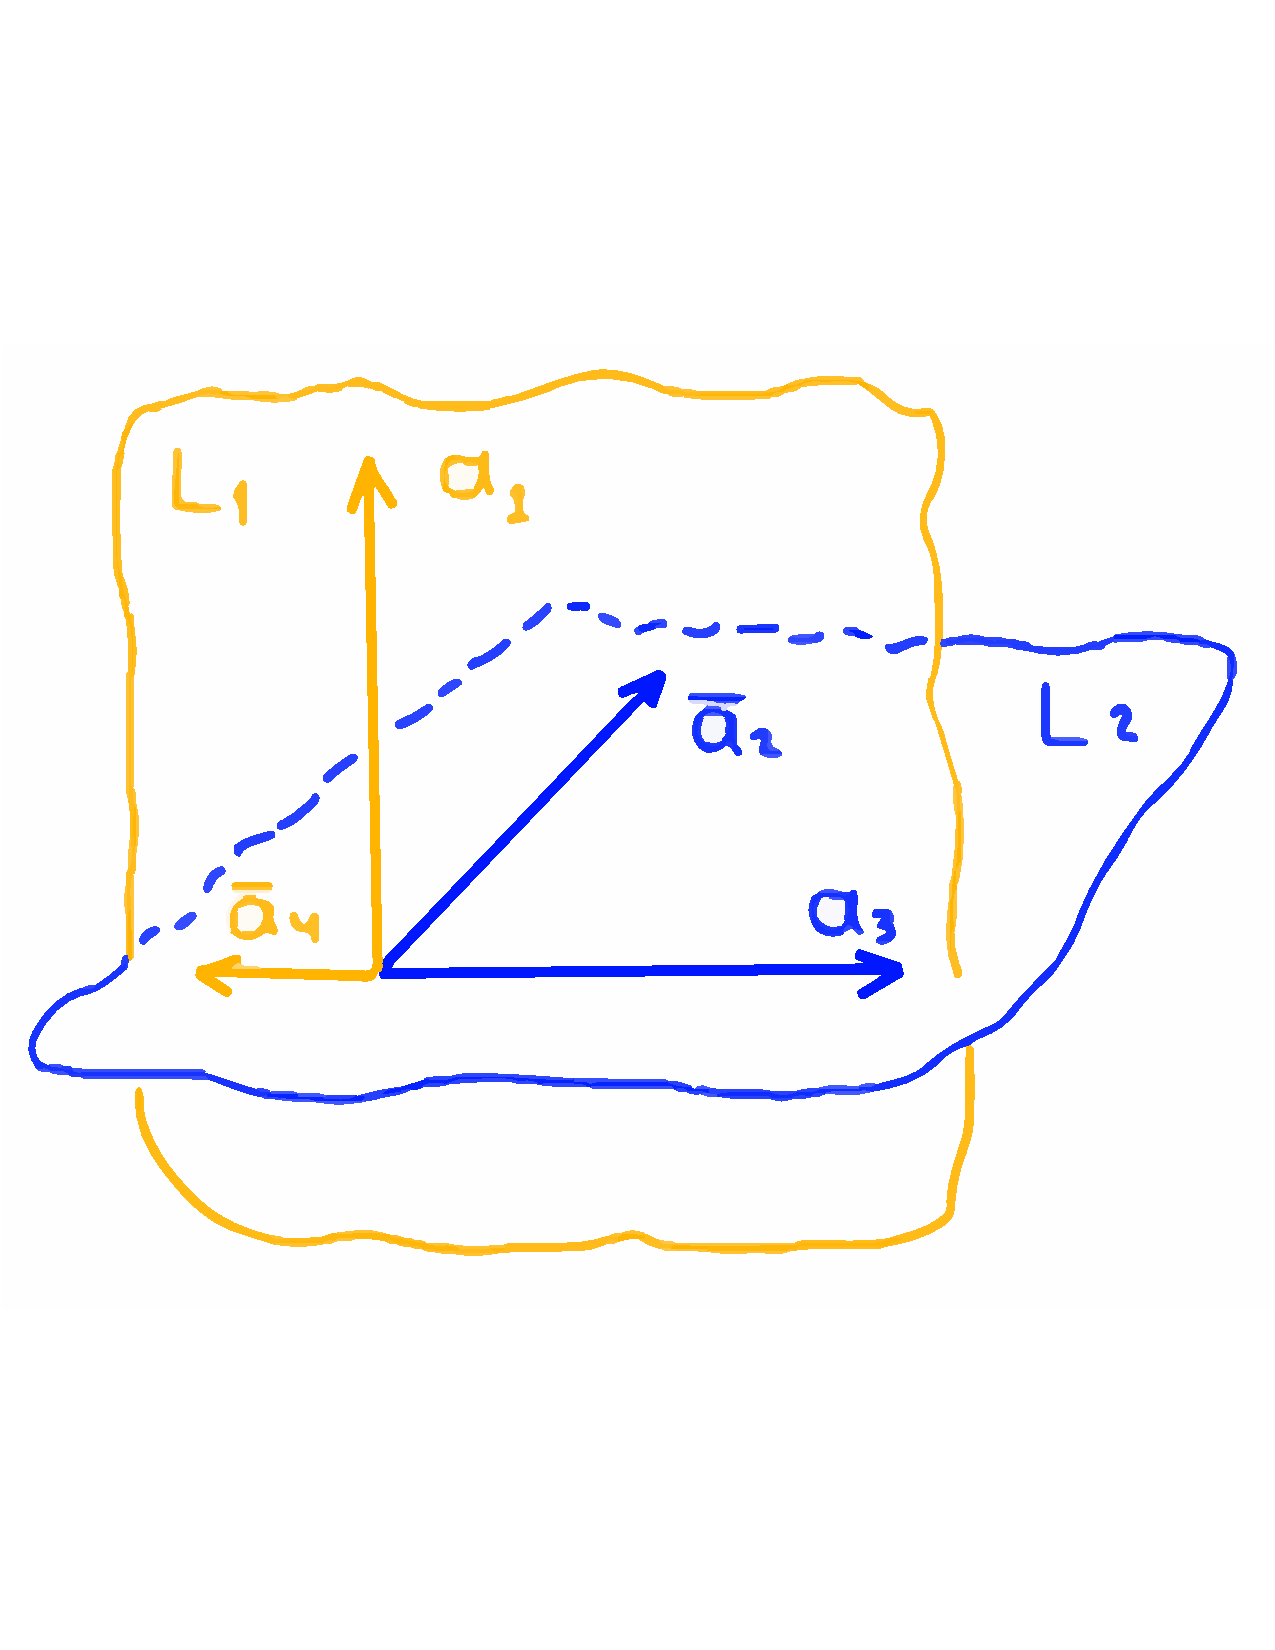
\includegraphics[width=0.8\linewidth]{sem/sem_4/prim_b_cvet} \\ б)}
	\end{minipage}
	\caption{Рисунки подпространств к примерам а) и б)}
	\label{ris:image1}
\end{figure}

\noindent а) ${\color{orange}L_1}\!:~ <\overline{a}_1\!> \qquad \dim L_1 = 1$\\
\phantom{а)}${\color{blue}L_2}\!:~ <\overline{a}_2, \overline{a}_3\!> \qquad \dim L_2 = 2$\\
В данном случае вектора некомпланарны.\\
$L_1+L_2=<\overline{a}_1, \overline{a}_2, \overline{a}_3\!> = \mathbb{R}^3$\\
$\dim (L_1 +L_2) = 3 = \dim L_1 + \dim L_2$\\
Т.о.
$$
L_1+L_2 = L_1 \oplus L_2
$$
%\begin{wrapfigure}{l}{0.3\linewidth}
%	\includegraphics[height=0.2\textheight]{prim_a_cvet}
%	\caption{Рисунок подпространств к примеру а)}
%\end{wrapfigure}
б) ${\color{orange}L_1}\!:~ <\overline{a}_1, \overline{a}_4> \qquad \dim L_1 = 2$\\
${\color{blue}L_2}\!:~ <\overline{a}_2, \overline{a}_3> \qquad \dim L_2 = 2$\\
$L_1+L_2\!:~<\overline{a}_1, \overline{a}_2, \overline{a}_3, \overline{a}_4\!>: \mathbb{R}^3$\\
Но $\dim (L_1+L_2)=3$, т.к. $\overline{a}_4$ можно выкинуть.

В общем случае:
$$
\dim (L_1+L_2) \leq \dim L_1 + \dim L_2
$$
Ответ о размерности даёт \textsf{формула Грассмана}:
$$
\dim (L_1+L_2)=\dim L_1+ \dim L_2 - \dim(L_1\cap L_2).
$$
\section{Понятие проекции вектора на подпространство}
\begin{definition}
	Пусть $\exists a\in L_1,\ b\in L_2, \ x \in L_1+L_2:\ \exists!x = a + b \Leftrightarrow L_1+L_2 = L_1 \oplus L_2$. При этом вектор $a$ называется \textsf{проекцией вектора} $x$ на $L_1$ параллельно $L_2$.  
\end{definition}
\begin{prim}
	Найти проекцию $X(0\ -1\ -1\ 4)^{\text{T}}$ на подпространство $L_1: x_1+x_2+x_3+x_4=0$ вдоль линейной оболочки $L_2\!:~<(1\ -1\ 1\ 0)^{\text{T}}$>.
\end{prim}\\
$L_1: (1\ 1\ 1\ 1\ |\ 0)\Rightarrow
\begin{pmatrix}
x_1\\
x_2\\
x_3\\
x_4\\
\end{pmatrix}
=
\begin{pmatrix*}[r]
-1&-1&-1\\
1&0&0\\
0&1&0\\
0&0&1\\
\end{pmatrix*}
\begin{pmatrix*}[r]
c_1\\
c_2\\
c_3\\
\end{pmatrix*}
$
или
$L_1:
<
\begin{pmatrix*}[r]
-1\\
1\\
0\\
0\\
\end{pmatrix*}
,
\begin{pmatrix*}[r]
-1\\
0\\
1\\
0\\
\end{pmatrix*}
,
\begin{pmatrix*}[r]
-1\\
0\\
0\\
1\\
\end{pmatrix*}
>.
$\\
$
L_2\!:~<\begin{pmatrixr}
1\\-1\\1\\0\\
\end{pmatrixr}>
$\\
Разложим вектор $X$:\\
$$
\begin{pmatrixr}
0\\-1\\-1\\4
\end{pmatrixr}
=\underbrace{
	k
	\begin{pmatrixr}
	1\\-1\\1\\0\\
	\end{pmatrixr}
}_{b\in L_2}
+\underbrace{
	\alpha
	\begin{pmatrixr}
	-1\\1\\0\\0\\
	\end{pmatrixr}
	+\beta
	\begin{pmatrixr}
	-1\\0\\1\\0\\
	\end{pmatrixr}
	+\gamma
	\begin{pmatrixr}
	4\\0\\0\\1\\
	\end{pmatrixr}
}_{a\in L_1}
$$
Очевидно, что это уравнение задает нам СЛУ. Составим ее расширенную матрицу и решим систему:\\
$
\left(\begin{array}{rrrr|r}
1&-1&-1&4&0\\
-1&1&0&0&-1\\
1&0&1&0&-1\\
0&0&0&1&4\\
\end{array}\right)
\rightarrow
\begin{pmatrixr}
k\\\alpha\\\beta\\\gamma\\
\end{pmatrixr}
=
\begin{pmatrixr}
2\\1\\-3\\4\\
\end{pmatrixr}.
$\\
Отсюда легко найти, что
$$
x_{\text{пр}}=
\begin{pmatrixr}
0\\-1\\-1\\4\\
\end{pmatrixr}
-2
\begin{pmatrixr}
1\\-1\\1\\0\\
\end{pmatrixr}
=
\begin{pmatrixr}
-2\\1\\-3\\4\\
\end{pmatrixr}.
$$

\begin{prim}
	Найти размероность и базис суммы подпространств $U_1$ и $U_2$.
	$$
	U_1\!:~<
	\begin{psm}
	1\\0\\-2\\0\\
	\end{psm}
	,
	\begin{psm}
	2\\1\\-1\\1
	\end{psm}
	,
	\begin{psm}
	3\\2\\0\\2
	\end{psm}
	>
	\quad
	U_2:
	\left\{
	\begin{array}{rrrrl}
	x_1&-2x_2&-3x_3&+4x_4&=0\\
	3x_1&+x_2&-2x_3&-2x_4&=0\\
	\end{array}
	\right.
	$$
\end{prim}
$
U_1:
\begin{pmatrixr}
1&0&-2&0\\
2&1&-1&1\\
3&2&0&2\\
\end{pmatrixr}
\xrightarrow[(3)-3(1)]{(2)-2(1)}
\begin{pmatrixr}
1&0&-2&0\\
0&1&3&1\\
0&2&6&2\\
\end{pmatrixr}
$\\
Последняя строка ЛЗ со второй, ее можно вычеркнуть $\Rightarrow \dim U_1 = 2$, базис:
$\left\{
\begin{psm}
1\\0\\-2\\0\\
\end{psm}
,
\begin{psm}
0\\1\\3\\1\\
\end{psm}
\right\}.
$\\
Переведём способ задания $U_2$ из СЛУ в линейную оболочку. Для этого решим эту СЛУ:\\
$
\left(\begin{array}{rrrrr}
1&-2&-3&4&0\\
3&1&-2&-2&0\\
\end{array}\right)
\rightarrow
\left(\begin{array}{rrrrr}
1&0&-1&0&0\\
0&1&1&-2&0\\
\end{array}\right)
$\\
$$
\begin{pmatrixr}
x_1\\x_2\\x_3\\x_4\\
\end{pmatrixr}
=
\begin{pmatrixr}
1&0\\
-1&2\\
1&0\\
0&1\\
\end{pmatrixr}
\begin{pmatrixr}
c_1\\c_2\\
\end{pmatrixr}, \quad \dim U_2 = 2, \quad \text{ базис }U_2:\left\{\begin{pmatrixr}
1\\-1\\1\\0\\
\end{pmatrixr}
,
\begin{pmatrixr}
0\\-2\\0\\1\\
\end{pmatrixr}\right\}.
$$
$
U_1+U_2\!:~<
\begin{psm}
1\\0\\-2\\0
\end{psm}
,
\begin{psm}
0\\1\\3\\1\\
\end{psm}
,\begin{psm}
1\\-1\\1\\0\\
\end{psm}
,
\begin{psm}
0\\2\\0\\1\\
\end{psm}
>.
$\\
$
\begin{pmatrixr}
1&0&1&0\\
0&1&-1&2\\
2&3&1&0\\
0&1&0&1\\
\end{pmatrixr}
\xrightarrow{(3)-(1)}
\begin{pmatrixr}
1&0&-&2&0\\
0&1&3&1\\
0&-1&3&0\\
0&2&0&1\\
\end{pmatrixr}
$\\
3 строка ЛЗ с 2 и 4, ее можно вычеркнуть $\Rightarrow \dim(U_1+U_2) = 3$, базис:
$
\left\{
\begin{psm}
1\\0\\-2\\0\\
\end{psm}
,
\begin{psm}
0\\1\\3\\1\\
\end{psm}
,
\begin{psm}
0\\2\\0\\1\\
\end{psm}
\right\}.
$
\begin{prim}
	В условиях примера 4 найти размерность и базис пересечения.
\end{prim}\\
$\dim  (U_1+U_2)=\dim  U_1+\dim  U_2-\dim (U_1 \cap U_2)$\\
$\dim  (U_1+U_2)=3$, $\dim  U_1=2$, $\dim  U_2=2 \Rightarrow \dim (U_1 \cap U_2)=1$

\noindent\textbf{1 способ}

Зададим $U_1$ как систему: 
$U_1\!:~<\left(
\begin{smallmatrix*}[r]
1\\
0\\
-2\\
0\\
\end{smallmatrix*}
\right) , \left(
\begin{smallmatrix*}[r]
0\\
1\\
3\\
1\\
\end{smallmatrix*}
\right)>$\\
$$
\begin{pmatrix*}[r]
1 & 0 & \vrule & x_1\\
0 & 1 & \vrule & x_2\\
-2 & 3 & \vrule & x_3\\
0 & 1 & \vrule & x_4\\
\end{pmatrix*}
\xrightarrow[(4)-(2)]{ 
	(3)+2(1),
	(3)-3(2)}
\begin{pmatrix*}[c]
1 & 0 & \vrule & x_1\\
0 & 1 & \vrule & x_2\\
0 & 0 & \vrule & x_3+2x_1-3x_2\\
0 & 0 & \vrule & x_4-x_2\\
\end{pmatrix*}
$$\\
$
U_1: 
\left\{	
\begin{array}{rrrrl}
2x_1 & - 3x_2 & + x_3 & & =0 \\
2x_1 & + x_2 & & + x_4 & =0 \\
\end{array}
\right.
$\\
$
U_1 \cap U_2= 
\left\{	
\begin{array}{c}
U_1 \\
U_2 \\
\end{array}
\right.
$\\
$$
\begin{pmatrix*}[r]
1 & 0 & -1 & 0 & \vrule & 0\\
0 & 1 & 1 & -2 & \vrule & 0\\
2 & -3 & -1 & 0 & \vrule & 0\\
0 & -1 & 0 & 1& \vrule & 0\\
\end{pmatrix*}
\Rightarrow
<
\begin{pmatrix*}[c]
1\\
1\\
1\\
1\\
\end{pmatrix*}
> (\text{базис } U_1 \cap U_2)
$$
\textbf{2 способ}\\
Базис $U_1: a_1, a_2$\\
Базис $U_2: b_1, b_2$\\
$P \in U_1, P \in U_2;$ \\
$ P=\alpha_1a_1+\alpha_2a_2=\beta_1b_1+\beta_2b_2 \Rightarrow \alpha_1, \alpha_2 $



